% ================================================================
% Section VII-F: MDEAS Scheduler Decision Space
% IEEE VTC Fall 2026 — Post-Quantum UAV Secure Communication
% Data: SCHEDULER_DECISION_SPACE.tex + SCHEDULER_SUITE_INSIGHTS.tex
% Palette: Paul Tol — ptblue=#004488, ptgold=#DDAA33, ptrose=#BB5566
% ================================================================

\subsection{MDEAS Scheduler Decision Space}
\label{sec:scheduler}

The preceding sections established individual component performance in
isolation.  This subsection synthesises those results into the
\emph{complete} operational decision space that the Multi-Dimensional
Energy-Aware Scheduler (MDEAS) must navigate in real time.  We formalise
the 27-point operating matrix, the forbidden-combination registry, the
9-gate priority cascade, and the 11-action inventory before analysing
suite-level Pareto trade-offs, rekey sustainability, and compound
constraint interactions.  The analysis reveals that MDEAS is not a
simple threshold controller but a priority cascade with cross-axis
feedback, where thermal budget---not cryptographic cost---is the binding
constraint.

%% ---------------------------------------------------------------
%% TABLE 1: 27-POINT OPERATING MATRIX (3 AEAD × 3 Level × 3 Det)
%% ---------------------------------------------------------------
\begin{table*}[!t]
\centering
\caption{Complete MDEAS 3-Axis Operating-Point Matrix.
Twenty-seven combinations of AEAD$\,\times\,$NIST Level$\,\times\,$DDoS
Detector; three Ascon+TST cells are forbidden ($\Delta T=12.2$\,°C).}
\label{tab:sched_matrix}
\footnotesize
\setlength{\tabcolsep}{3pt}
\begin{tabular}{@{}ll ccc ccc ccc@{}}
\toprule
& & \multicolumn{3}{c}{\textbf{Detector = NONE}}
& \multicolumn{3}{c}{\textbf{Detector = XGBoost}}
& \multicolumn{3}{c}{\textbf{Detector = TST}} \\
\cmidrule(lr){3-5}\cmidrule(lr){6-8}\cmidrule(lr){9-11}
\textbf{AEAD} & \textbf{Metric}
 & \textbf{L1} & \textbf{L3} & \textbf{L5}
 & \textbf{L1} & \textbf{L3} & \textbf{L5}
 & \textbf{L1} & \textbf{L3} & \textbf{L5} \\
\midrule
\multirow{4}{*}{\rotatebox{90}{\textbf{ChaCha20}}}
 & Tier Score          & 1   & 11  & 21  & 1   & 11  & 21  & 1   & 11  & 21  \\
 & $\Delta$CPU (pp)    & 0   & 0   & 0   & +26 & +26 & +26 & +74 & +74 & +74 \\
 & $\Delta T$ (°C)     & 0   & 0   & 0   & +13 & +13 & +13 & +22 & +22 & +22 \\
 & Safe $T_\text{amb}$ & 80  & 80  & 80  & 67  & 67  & 67  & 58  & 58  & 58  \\
\midrule
\multirow{4}{*}{\rotatebox{90}{\textbf{AES-GCM}}}
 & Tier Score          & 0   & 10  & 20  & 0   & 10  & 20  & 0   & 10  & 20  \\
 & $\Delta$CPU (pp)    & 0   & 0   & 0   & +26 & +26 & +26 & +74 & +74 & +74 \\
 & $\Delta T$ (°C)     & 0   & 0   & 0   & +13 & +13 & +13 & +22 & +22 & +22 \\
 & Safe $T_\text{amb}$ & 80  & 80  & 80  & 67  & 67  & 67  & 58  & 58  & 58  \\
\midrule
\multirow{4}{*}{\rotatebox{90}{\textbf{Ascon}}}
 & Tier Score          & 2   & 12  & 22
   & 2   & 12  & 22
   & \cellcolor{ptrose!20}\textbf{---}
   & \cellcolor{ptrose!20}\textbf{---}
   & \cellcolor{ptrose!20}\textbf{---} \\
 & $\Delta$CPU (pp)    & 0   & 0   & 0   & +26 & +26 & +26
   & \cellcolor{ptrose!20}$\times$
   & \cellcolor{ptrose!20}$\times$
   & \cellcolor{ptrose!20}$\times$ \\
 & $\Delta T$ (°C)     & +1.5& +1.5& +1.5& +14 & +14 & +14
   & \cellcolor{ptrose!20}$\times$
   & \cellcolor{ptrose!20}$\times$
   & \cellcolor{ptrose!20}$\times$ \\
 & Safe $T_\text{amb}$ & 78.5& 78.5& 78.5& 66  & 66  & 66
   & \cellcolor{ptrose!20}Forbid
   & \cellcolor{ptrose!20}Forbid
   & \cellcolor{ptrose!20}Forbid \\
\bottomrule
\end{tabular}
\begin{flushleft}
\footnotesize
Tier $=$ NIST\_LEVEL\,$(0/10/20)$ + KEM\_COMPLEXITY + AEAD\_PERF\,$(0/1/2)$.
$T_\text{amb}$ is the maximum ambient temperature where
$T_\text{die}\leq80$\,°C (critical threshold).
Ascon+TST combined $\Delta T = 1.5 + 10.7 = 12.2$\,°C exceeds the
safe thermal margin.
\end{flushleft}
\end{table*}

\subsubsection{Operating-Point Enumeration}
The MDEAS control space is defined by three orthogonal axes---AEAD
cipher (ChaCha20-Poly1305, AES-256-GCM, Ascon-128a), NIST security
level (L1/L3/L5), and DDoS detector (NONE/XGBoost/TST)---yielding
$3\times3\times3=27$ operating points.
Table~\ref{tab:sched_matrix} presents the complete matrix.  Each cell
records the tier score (scheduler priority), marginal CPU load
($\Delta$\,pp), thermal delta ($\Delta T$), and maximum safe ambient
temperature.  Twenty-four of the 27 points are viable; the three
Ascon+TST cells are \emph{forbidden} because the compound thermal
delta of \SI{12.2}{\degreeCelsius} exceeds the RPi4's safe margin at
typical UAV ambient temperatures (\SIrange{45}{55}{\degreeCelsius}).

%% ---------------------------------------------------------------
%% TABLE 2: FORBIDDEN COMBINATION REGISTRY
%% ---------------------------------------------------------------
\begin{table}[!t]
\centering
\caption{Forbidden Combination Registry.
Three empirically-derived exclusions enforced at policy level reduce
the 648 theoretical configurations to ${\approx}\,500$ viable states.}
\label{tab:sched_forbidden}
\footnotesize
\setlength{\tabcolsep}{3pt}
\begin{tabular}{@{}lll@{}}
\toprule
\textbf{Combination} & \textbf{Constraint} & \textbf{Mechanism} \\
\midrule
Ascon-128a + TST & Thermal: $\Delta T=12.2$\,°C & Policy forbid list \\
McEliece + TST   & CPU contention: keygen $>$\SI{134}{\ms} & Policy forbid list \\
McEliece + SPHINCS+ & HS timeout: $T_\text{HS}>45$\,s & Suite validation \\
\midrule
\multicolumn{3}{@{}l}{\textit{Impact: 648 theoretical $\to$ ${\approx}\,500$
viable (${\approx}\,23\%$ reduction)}} \\
\bottomrule
\end{tabular}
\end{table}

The three forbidden combinations (Table~\ref{tab:sched_forbidden})
emerge from \emph{empirical} measurement, not theoretical assumptions:
(i)~Ascon-128a+TST produces a compound thermal delta of
\SI{12.2}{\degreeCelsius} that overshoots the \SI{80}{\degreeCelsius}
critical threshold at any ambient above \SI{58}{\degreeCelsius};
(ii)~McEliece+TST creates CPU contention during key generation
($>$\SI{134}{\ms} at 88.8\% CPU), starving the transport layer;
(iii)~McEliece+SPHINCS+ handshakes exceed the
\SI{45}{\second} timeout (MC460+SP192s measured at
\SI{48.2}{\second}).  Together these exclusions eliminate
${\approx}\,23\%$ of the theoretical space.

%% ---------------------------------------------------------------
%% FIGURE 1: 9-GATE DECISION CASCADE FLOWCHART
%% ---------------------------------------------------------------
\begin{figure*}[!t]
\centering
\begin{tikzpicture}[
    node distance=0.45cm and 0.8cm,
    box/.style={draw, rounded corners, minimum height=0.6cm,
      minimum width=2cm, font=\scriptsize, align=center, inner sep=2pt},
    decision/.style={draw, diamond, aspect=2.2, minimum width=1.4cm,
      font=\scriptsize, align=center, inner sep=1pt},
    act_crit/.style={draw, fill=ptrose!20, rounded corners,
      minimum height=0.5cm, font=\scriptsize\bfseries, inner sep=2pt},
    act_warn/.style={draw, fill=ptgold!25, rounded corners,
      minimum height=0.5cm, font=\scriptsize\bfseries, inner sep=2pt},
    act_safe/.style={draw, fill=ptblue!15, rounded corners,
      minimum height=0.5cm, font=\scriptsize\bfseries, inner sep=2pt},
    act_hold/.style={draw, fill=ptgray!15, rounded corners,
      minimum height=0.5cm, font=\scriptsize\bfseries, inner sep=2pt},
    arr/.style={-{stealth}, thick},
    yarr/.style={-{stealth}, thick, ptgold!80!black},
    rarr/.style={-{stealth}, thick, ptrose},
]
% Gate 1 — telemetry stale
\node[decision] (g1) {Telemetry\\stale $>2$\,s?};
\node[act_hold, right=0.6cm of g1] (a1) {HOLD};
\draw[rarr] (g1) -- node[above,font=\tiny]{Y} (a1);
\node[right=0.1cm of a1, font=\tiny\itshape, text=ptgray] {wait for data};

% Gate 2 — emergency
\node[decision, below=0.45cm of g1] (g2) {Batt$<$\SI{14}{\kilo\volt}\\or $T>$\SI{80}{\degreeCelsius}?};
\node[act_crit, right=0.6cm of g2] (a2) {EMERGENCY};
\draw[rarr] (g2) -- node[above,font=\tiny]{Y} (a2);
\draw[arr] (g1) -- node[left,font=\tiny]{N} (g2);
\node[right=0.1cm of a2, font=\tiny\itshape, text=ptrose] {max downgrade};

% Gate 3 — DDoS
\node[decision, below=0.45cm of g2] (g3) {DDoS\\detected?};
\node[act_crit, right=0.6cm of g3] (a3) {EMERGENCY};
\draw[rarr] (g3) -- node[above,font=\tiny]{Y} (a3);
\draw[arr] (g2) -- node[left,font=\tiny]{N} (g3);
\node[right=0.1cm of a3, font=\tiny\itshape, text=ptrose] {threat response};

% Gate 4 — detector thermal
\node[decision, below=0.45cm of g3] (g4) {Detector\\thermal\\conflict?};
\node[act_warn, right=0.6cm of g4] (a4) {DOWNGRADE\_DET};
\draw[yarr] (g4) -- node[above,font=\tiny]{Y} (a4);
\draw[arr] (g3) -- node[left,font=\tiny]{N} (g4);
\node[right=0.1cm of a4, font=\tiny\itshape, text=ptgold!80!black]
  {TST$\to$XGB$\to$NONE};

% Gate 5 — predictive thermal
\node[decision, below=0.45cm of g4] (g5) {Predictive\\$T$ rising?};
\node[act_warn, right=0.6cm of g5] (a5) {SWITCH\_AEAD};
\draw[yarr] (g5) -- node[above,font=\tiny]{Y} (a5);
\draw[arr] (g4) -- node[left,font=\tiny]{N} (g5);
\node[right=0.1cm of a5, font=\tiny\itshape, text=ptgold!80!black]
  {Ascon$\to$ChaCha};

% Gate 6 — battery stress
\node[decision, below=0.45cm of g5] (g6) {Battery\\drain high?};
\node[act_warn, right=0.6cm of g6] (a6) {SWITCH\_AEAD};
\draw[yarr] (g6) -- node[above,font=\tiny]{Y} (a6);
\draw[arr] (g5) -- node[left,font=\tiny]{N} (g6);
\node[right=0.1cm of a6, font=\tiny\itshape, text=ptgold!80!black]
  {lower $\mu$s cipher};

% Gate 7 — link
\node[decision, below=0.45cm of g6] (g7) {Link\\degraded?};
\node[act_warn, right=0.6cm of g7] (a7) {DOWNGRADE\_LVL};
\draw[yarr] (g7) -- node[above,font=\tiny]{Y} (a7);
\draw[arr] (g6) -- node[left,font=\tiny]{N} (g7);
\node[right=0.1cm of a7, font=\tiny\itshape, text=ptgold!80!black]
  {L5$\to$L3$\to$L1};

% Gate 8 — rekey
\node[decision, below=0.45cm of g7] (g8) {Rekey\\interval?};
\node[act_safe, right=0.6cm of g8] (a8) {REKEY};
\draw[arr] (g8) -- node[above,font=\tiny]{Y} (a8);
\draw[arr] (g7) -- node[left,font=\tiny]{N} (g8);
\node[right=0.1cm of a8, font=\tiny\itshape, text=ptblue]
  {proactive rotate};

% Gate 9 — stable upgrade
\node[decision, below=0.45cm of g8] (g9) {Stable\\$>30$\,s?};
\node[act_safe, right=0.6cm of g9] (a9) {UPGRADE\_LVL};
\draw[arr] (g9) -- node[above,font=\tiny]{Y} (a9);
\draw[arr] (g8) -- node[left,font=\tiny]{N} (g9);
\node[right=0.1cm of a9, font=\tiny\itshape, text=ptblue]
  {L1$\to$L3$\to$L5};

% Default HOLD
\node[act_hold, below=0.45cm of g9] (a10) {HOLD};
\draw[arr] (g9) -- node[left,font=\tiny]{N} (a10);
\end{tikzpicture}
\caption{MDEAS 9-gate priority cascade (EnergyAwarePolicy).
Each gate is evaluated in strict order; first match wins.
Gates~1--3 (red) handle safety-critical conditions and bypass all
hysteresis timers.  Gates~4--7 (gold) address thermal and resource
stress with rate-based predictive sub-checks.  Gates~8--9 (blue)
perform proactive maintenance when the system is stable.}
\label{fig:sched_cascade}
\end{figure*}

\subsubsection{Decision Cascade Architecture}
Fig.~\ref{fig:sched_cascade} presents the 9-gate priority cascade
that constitutes the MDEAS decision engine.  The cascade evaluates
gates in strict order---telemetry freshness, emergency, DDoS, detector
thermal conflict, predictive thermal, AEAD stress, battery drain, link
quality, rekey interval, and stable upgrade---with first-match semantics.
Emergency conditions (Gates~1--3) bypass all \SI{5}{\second} hysteresis
timers, ensuring sub-second response to critical events.  The
predictive thermal module (Gate~5) projects die temperature
\SI{60}{\second} forward using rate-of-change data, enabling
pre-emptive AEAD switching before the \SI{80}{\degreeCelsius} threshold
is reached.

%% ---------------------------------------------------------------
%% TABLE 3: ENVIRONMENTAL TRIGGER ZONES
%% ---------------------------------------------------------------
\begin{table}[!t]
\centering
\caption{Environmental Trigger Zones and Scheduler Responses.
Four sensor domains, 18 trigger conditions, and two rate-of-change
predictors feed the 9-gate cascade.}
\label{tab:sched_triggers}
\footnotesize
\setlength{\tabcolsep}{2.5pt}
\begin{tabular}{@{}ll>{\raggedright\arraybackslash}p{2.9cm}l@{}}
\toprule
\textbf{Sensor} & \textbf{Zone} & \textbf{Condition} & \textbf{Action} \\
\midrule
\multirow{4}{*}{Battery}
 & \cellcolor{ptblue!8}Normal
   & $V > 15200$\,mV & HOLD / UPGRADE \\
 & \cellcolor{ptgold!12}Warn
   & $14800 < V \leq 15200$\,mV & SWITCH\_AEAD \\
 & \cellcolor{ptgold!12}Low
   & $14000 < V \leq 14800$\,mV & DOWNGRADE \\
 & \cellcolor{ptrose!12}Critical
   & $V \leq 14000$\,mV & EMERGENCY \\
\midrule
\multirow{3}{*}{\shortstack[l]{Battery\\Drain}}
 & \cellcolor{ptblue!8}Normal
   & $\dot{V} < 200$\,mV/min & HOLD \\
 & \cellcolor{ptgold!12}Fast
   & $200 \leq \dot{V} < 500$\,mV/min & SWITCH\_AEAD \\
 & \cellcolor{ptrose!12}Critical
   & $\dot{V} \geq 500$\,mV/min  & DOWNGRADE \\
\midrule
\multirow{3}{*}{Thermal}
 & \cellcolor{ptblue!8}Normal
   & $T < 70$\,°C & HOLD / UPGRADE \\
 & \cellcolor{ptgold!12}Warn
   & $70 \leq T < 80$\,°C & SWITCH\_AEAD \\
 & \cellcolor{ptrose!12}Critical
   & $T \geq 80$\,°C & EMERGENCY \\
\midrule
\multirow{2}{*}{\shortstack[l]{Thermal\\Rate}}
 & \cellcolor{ptblue!8}Normal
   & $\dot{T} < 5$\,°C/min & HOLD \\
 & \cellcolor{ptgold!12}Rising
   & $\dot{T} \geq 5$\,°C/min & SWITCH\_AEAD \\
\midrule
\multirow{3}{*}{Link}
 & \cellcolor{ptblue!8}Good
   & pps $\geq 5$, gap $< 1$\,s & HOLD / UPGRADE \\
 & \cellcolor{ptgold!12}Degraded
   & pps $< 5$ or gap $\geq 1$\,s & DOWNGRADE\_LVL \\
 & \cellcolor{ptrose!12}Blackout
   & $\geq 3$ consec.\ blackouts & ROLLBACK \\
\midrule
\multirow{2}{*}{Rekey}
 & \cellcolor{ptblue!8}Fresh
   & age $<$ interval, window ok & HOLD \\
 & \cellcolor{ptgold!12}Due
   & age $\geq$ interval, stable $>10$\,s & REKEY \\
\midrule
DDoS
 & \cellcolor{ptrose!12}Active
   & Detector alert fired & EMERGENCY \\
\bottomrule
\end{tabular}
\end{table}

%% ---------------------------------------------------------------
%% TABLE 4: 11-ACTION INVENTORY
%% ---------------------------------------------------------------
\begin{table}[!t]
\centering
\caption{Complete MDEAS Action Inventory.
Eleven actions span three control axes (AEAD, Level, Detector) plus
global overrides; each action's trigger, axis, and direction are
defined deterministically by the cascade.}
\label{tab:sched_actions}
\footnotesize
\setlength{\tabcolsep}{2.5pt}
\begin{tabular}{@{}l>{\raggedright\arraybackslash}p{2.5cm}ll@{}}
\toprule
\textbf{Action} & \textbf{Trigger} & \textbf{Axis} & \textbf{Direction} \\
\midrule
HOLD            & No trigger / cooldown    & ---   & --- \\
EMERGENCY       & $V<14$\,kV, $T>80$°C, DDoS & All & Max downgrade \\
SWITCH\_AEAD    & Thermal/battery pressure & AEAD  & Lower cost \\
DOWNGRADE\_LVL  & Link degraded            & Level & L5$\to$L3$\to$L1 \\
UPGRADE\_LVL    & Stable $>30$\,s          & Level & L1$\to$L3$\to$L5 \\
DOWNGRADE\_DET  & Det.\ thermal conflict   & Det.  & TST$\to$XGB$\to$NONE \\
UPGRADE\_DET    & Threat + headroom        & Det.  & NONE$\to$XGB$\to$TST \\
REKEY           & Interval elapsed+stable  & ---   & Key rotation \\
DOWNGRADE       & Battery/link stress      & Suite & Lower tier \\
UPGRADE         & Stable + disarmed        & Suite & Higher tier \\
ROLLBACK        & Link fail + recent switch& Suite & Previous suite \\
\bottomrule
\end{tabular}
\end{table}

Table~\ref{tab:sched_triggers} enumerates the environmental trigger
zones across battery (4 zones), thermal (3), link (3), rekey (2), and
DDoS (1) domains, while Table~\ref{tab:sched_actions} catalogues the
complete 11-action inventory.  The actions are not independent:
EMERGENCY simultaneously drives all three axes to their minimum-cost
settings, always targeting ML512+F512+ChaCha20+NONE (Tier~1).

%% ---------------------------------------------------------------
%% TABLE 5: 18 SUITE BUILDING BLOCKS
%% ---------------------------------------------------------------
\begin{table*}[!t]
\centering
\caption{Suite Building Blocks: 18 Components and Scheduler Implications.
From these primitives the system generates 72 valid suites; the
scheduler must navigate this space under real-time constraints.}
\label{tab:sched_taxonomy}
\footnotesize
\setlength{\tabcolsep}{3pt}
\begin{tabular}{@{}llrrrrl@{}}
\toprule
\textbf{Component} & \textbf{Type}
& \textbf{Key Cost}
& \textbf{PK/CT/Sig\,(B)}
& \textbf{NIST}
& \textbf{Tier Add}
& \textbf{Scheduler Implication} \\
\midrule
ML-KEM-512   & KEM & $<1$\,ms   & 800\,/\,768\,/\,--- & L1 & +0
  & Fastest KEM; rekey-friendly \\
ML-KEM-768   & KEM & $<1$\,ms   & 1184\,/\,1088\,/\,--- & L3 & +0
  & Default recommendation \\
ML-KEM-1024  & KEM & $<1$\,ms   & 1568\,/\,1568\,/\,--- & L5 & +0
  & Negligible overhead vs 768 \\
HQC-128      & KEM & ${\approx}50$\,ms   & 4522\,/\,8978\,/\,--- & L1 & +3
  & $50{\times}$ slower; link-sensitive \\
HQC-192      & KEM & ${\approx}155$\,ms  & ---\,/\,---\,/\,---   & L3 & +3
  & Significant rekey cost \\
HQC-256      & KEM & ${\approx}272$\,ms  & ---\,/\,---\,/\,---   & L5 & +3
  & Heavy; $\Phi>0.9\%$ at $R{=}30$\,s \\
McEliece-348 & KEM & ${\approx}190$\,ms  & \textbf{524\,kB PK} & L1 & +5
  & Bandwidth-prohibitive \\
McEliece-460 & KEM & ${\approx}257$\,ms  & \textbf{524\,kB PK} & L3 & +5
  & TST forbidden (CPU) \\
McEliece-8192& KEM & ${\approx}600$\,ms  & \textbf{1.36\,MB PK}& L5 & +5
  & TST forbidden; BW-prohibitive \\
\midrule
Falcon-512    & SIG & $<0.1$\,ms & ---\,/\,---\,/\,659  & L1 & ---
  & Fastest SIG at L1 \\
Falcon-1024   & SIG & $<0.1$\,ms & ---\,/\,---\,/\,1280 & L5 & ---
  & Fastest SIG at L5 \\
ML-DSA-44     & SIG & $<0.1$\,ms & ---\,/\,---\,/\,2420 & L1 & ---
  & $3.6{\times}$ larger sig vs Falcon \\
ML-DSA-65     & SIG & $<0.1$\,ms & ---\,/\,---\,/\,3309 & L3 & ---
  & Default L3 recommendation \\
ML-DSA-87     & SIG & $<0.1$\,ms & ---\,/\,---\,/\,4627 & L5 & ---
  & $3.6{\times}$ larger sig vs Falcon-1024 \\
SPHINCS+-128s & SIG & ${\approx}644$\,ms  & ---\,/\,---\,/\,7856  & L1 & ---
  & HS time dominated by SIG \\
SPHINCS+-192s & SIG & ${\approx}1233$\,ms & ---\,/\,---\,/\,16224 & L3 & ---
  & McEliece combo = timeout \\
SPHINCS+-256s & SIG & ${\approx}1092$\,ms & ---\,/\,---\,/\,29792 & L5 & ---
  & Large signature; link stress \\
\midrule
AES-256-GCM     & AEAD & \SI{67}{\micro\second} & --- & --- & +0
  & Lowest tier; HW-accel on x86 \\
ChaCha20-P1305  & AEAD & \SI{64}{\micro\second} & --- & --- & +1
  & Slightly faster on ARM \\
Ascon-128a      & AEAD & \SI{1327}{\micro\second}& --- & --- & +2
  & $20{\times}$ overhead; TST-forbidden \\
\bottomrule
\end{tabular}
\end{table*}

%% ---------------------------------------------------------------
%% FIGURE 2: SECURITY–PERFORMANCE PARETO FRONTIER
%% ---------------------------------------------------------------
\begin{figure}[!t]
\centering
\begin{tikzpicture}
\begin{axis}[
    width=\columnwidth,
    height=6.5cm,
    xlabel={Handshake Time (ms, log scale)},
    ylabel={NIST Security Level},
    xmode=log,
    xmin=5, xmax=60000,
    ymin=0.5, ymax=5.5,
    ytick={1,3,5},
    grid=major,
    legend style={at={(0.02,0.98)}, anchor=north west, font=\scriptsize,
      legend columns=1},
]
% ML-KEM suites (Pareto-optimal frontier)
\addplot[only marks, mark=*, mark size=3.5pt,
  color=ptblue, fill=ptblue!30] coordinates {
    (8.75,5)(8.79,5)(8.84,5)(11.13,5)(12.07,1)(12.09,1)(12.26,3)
    (12.71,3)(12.80,1)(13.16,3)(14.34,1)(14.40,5)(16.78,5)(18.88,5)
};
% HQC suites
\addplot[only marks, mark=square*, mark size=3pt,
  color=ptgold, fill=ptgold!30] coordinates {
    (54.75,1)(54.79,1)(57.80,1)(60.78,1)(60.81,1)(61.43,1)
    (154.5,3)(155.1,3)(155.8,3)
    (271.7,5)(276.1,5)(285.2,5)
};
% McEliece suites
\addplot[only marks, mark=triangle*, mark size=3.5pt,
  color=ptrose, fill=ptrose!30] coordinates {
    (124.1,1)(150.4,1)(187.5,1)(206.1,1)(206.2,1)
    (257.4,3)(304.9,3)
    (505.3,5)(507.1,5)(507.5,5)(678.4,5)(678.8,5)
};
% SPHINCS+ dominated region
\addplot[only marks, mark=diamond*, mark size=2.5pt,
  color=ptgray, fill=ptgray!30] coordinates {
    (655.1,1)(722.8,1)(1079.9,1)
    (1249.5,3)(1337.5,3)(1425.4,3)(1537.0,3)(1537.3,3)
    (1624.0,3)(2040.8,3)(48186,3)
    (1110.2,5)(1110.6,5)(1469.9,5)(1549.0,5)(1650.8,5)
    (1650.8,5)(2161.5,5)(2269.1,5)
};
% Pareto frontier line
\addplot[thick, dashed, black!70, mark=none] coordinates {
    (8.75,5)(12.80,1)
};
\node[font=\tiny\bfseries, anchor=south west, black!70]
  at (axis cs:9.5,4.4) {Pareto front};
% Key annotations
\node[font=\tiny, ptblue, anchor=west]
  at (axis cs:10,5.25) {ML1024+F1024};
\node[font=\tiny, ptblue, anchor=east]
  at (axis cs:12,0.75) {ML512+F512};
\node[font=\tiny, ptgray, anchor=west]
  at (axis cs:50000,3.25) {MC460+SP192};
\legend{ML-KEM, HQC, McEliece, SPHINCS+ combos}
\end{axis}
\end{tikzpicture}
\caption{Security--performance Pareto frontier across 72~suites.
The Pareto-optimal set (dashed) is \emph{exclusively} ML-KEM-based:
ML1024+F1024 achieves L5 in \SI{8.7}{\ms} while ML512+F512 achieves L1
in \SI{12.8}{\ms}.  HQC offers no Pareto advantage.  The entire
SPHINCS+ cluster ($>$\SI{600}{\ms}) provides no additional security
benefit over Falcon/ML-DSA alternatives at the same NIST level.}
\label{fig:sched_pareto}
\end{figure}

\subsubsection{Suite-Level Pareto Analysis}
Fig.~\ref{fig:sched_pareto} plots all 72~suites in the
security--performance plane.  The Pareto frontier is \emph{exclusively}
ML-KEM-based: ML1024+Falcon-1024 achieves L5 security in
\SI{8.7}{\ms}, and ML512+Falcon-512 achieves L1 in \SI{12.8}{\ms}.
Neither HQC nor McEliece offers a Pareto advantage---they are
strictly dominated at every NIST level.  The SPHINCS+ cluster
($>$\SI{600}{\ms}) provides identical NIST levels to Falcon/ML-DSA
alternatives but at $50$--$5500{\times}$ higher latency.

%% ---------------------------------------------------------------
%% TABLE 6: SUITE FAMILY PERFORMANCE PROFILES
%% ---------------------------------------------------------------
\begin{table}[!t]
\centering
\caption{Suite Family Performance Profiles (baseline, mean per family).
ML-KEM+fast SIG spans only $2.2{\times}$; McEliece+SPHINCS+ spans
$44.6{\times}$ with one timeout case---a scheduling nightmare.}
\label{tab:sched_families}
\footnotesize
\setlength{\tabcolsep}{2.5pt}
\begin{tabular}{@{}l r r r r r@{}}
\toprule
\textbf{KEM Family} & $n$ & $\overline{T}_\text{HS}$
& $T_\text{HS}^\text{min}$ & $T_\text{HS}^\text{max}$ & \textbf{Span} \\
\midrule
\multicolumn{6}{@{}l}{\textit{With fast SIG (Falcon/ML-DSA):}} \\
ML-KEM+fast   & 18 & 12.8\,ms   & 8.7\,ms  & 18.9\,ms  & $2.2{\times}$ \\
HQC+fast      & 12 & 140.2\,ms  & 54.7\,ms & 285.2\,ms & $5.2{\times}$ \\
McEliece+fast & 12 & 356.5\,ms  & 124.1\,ms& 678.4\,ms & $5.5{\times}$ \\
\midrule
\multicolumn{6}{@{}l}{\textit{With SPHINCS+:}} \\
ML-KEM+SP     & 6  & 1106.3\,ms & 655.1\,ms& 1337.5\,ms& $2.0{\times}$ \\
HQC+SP        & 6  & 1293.4\,ms & 722.8\,ms& 1624.0\,ms& $2.2{\times}$ \\
McEliece+SP   & 6  & 8442.3\,ms & 1079.9\,ms&48186\,ms & $44.6{\times}$ \\
\bottomrule
\end{tabular}
\end{table}

Table~\ref{tab:sched_families} quantifies the performance-span
contrast.  ML-KEM\,+\,fast~SIG suites span only $2.2{\times}$
(\SIrange{8.7}{18.9}{\ms}), making them \emph{highly predictable} for
the scheduler: all 18~variants complete within a single
\SI{30}{\second} rekey window with negligible overhead.  In stark
contrast, McEliece+SPHINCS+ spans $44.6{\times}$
(\SIrange{1.08}{48.2}{\second})---the scheduler cannot even predict
whether a handshake will complete before the timeout.

%% ---------------------------------------------------------------
%% FIGURE 3: HS TIME DECOMPOSITION STACKED BARS
%% ---------------------------------------------------------------
\begin{figure}[!t]
\centering
\begin{tikzpicture}
\begin{axis}[
    width=\columnwidth,
    height=6.5cm,
    xbar stacked,
    bar width=7pt,
    xlabel={Handshake Time (ms)},
    xmin=0, xmax=700,
    symbolic y coords={
        ML1024+F1024, ML768+DSA65, ML512+F512,
        HQ128+F512, HQ192+DSA65, HQ256+DSA87,
        MC348+DSA44, MC460+DSA65, MC8192+DSA87
    },
    ytick=data,
    yticklabel style={font=\tiny},
    legend style={at={(0.5,-0.16)}, anchor=north, legend columns=3,
      font=\scriptsize},
    enlarge y limits=0.12,
]
% KEM time
\addplot[fill=ptblue!60, draw=ptblue!80] coordinates {
    (1,ML1024+F1024)(1,ML768+DSA65)(0.8,ML512+F512)
    (50,HQ128+F512)(155,HQ192+DSA65)(272,HQ256+DSA87)
    (130,MC348+DSA44)(185,MC460+DSA65)(370,MC8192+DSA87)
};
% SIG time
\addplot[fill=ptgold!60, draw=ptgold!80] coordinates {
    (0.1,ML1024+F1024)(0.1,ML768+DSA65)(0.1,ML512+F512)
    (0.1,HQ128+F512)(0.1,HQ192+DSA65)(0.1,HQ256+DSA87)
    (0.1,MC348+DSA44)(0.1,MC460+DSA65)(0.1,MC8192+DSA87)
};
% TLS/network overhead
\addplot[fill=ptgray!40, draw=ptgray!60] coordinates {
    (7.6,ML1024+F1024)(10,ML768+DSA65)(7.1,ML512+F512)
    (7.7,HQ128+F512)(0.7,HQ192+DSA65)(3.9,HQ256+DSA87)
    (57.4,MC348+DSA44)(72.3,MC460+DSA65)(135,MC8192+DSA87)
};
\legend{KEM, SIG, TLS/Network}
\end{axis}
\node[font=\scriptsize, anchor=west] at (0,-3.6) {%
  \textit{Omitted}: SPHINCS+ combos ($>1$\,s, SIG-dominated)};
\end{tikzpicture}
\caption{Handshake time decomposition for fast-SIG suites.
ML-KEM handshakes are dominated by TLS overhead ($<1$\,ms KEM);
HQC by KEM cost (\SIrange{50}{272}{\ms}); McEliece by KEM plus
bandwidth-induced TLS overhead (\SIrange{130}{530}{\ms}).
SPHINCS+ combos are omitted ($>1$\,s, SIG-dominated).
This decomposition shows that AEAD switching cannot help
KEM-dominated suites---the scheduler must change KEM family instead.}
\label{fig:sched_decomp}
\end{figure}

%% ---------------------------------------------------------------
%% TABLE 7: REKEY SUSTAINABILITY Φ(R=30s)
%% ---------------------------------------------------------------
\begin{table}[!t]
\centering
\caption{Rekey Sustainability by Suite Category.
$\Phi(R)\!=\!T_\text{HS}/(R+T_\text{HS})$ represents the fraction of
time spent in handshake; ML-KEM suites sustain aggressive \SI{30}{\second}
rekey with $\Phi<0.06\%$, while MC460+SP192 is unusable ($\Phi=61.6\%$).}
\label{tab:sched_rekey}
\footnotesize
\setlength{\tabcolsep}{3pt}
\begin{tabular}{@{}l r r r l@{}}
\toprule
\textbf{Suite Category}
& $T_\text{HS}$
& $\Phi_{30\text{s}}$
& $\Phi_{300\text{s}}$
& \textbf{Verdict} \\
\midrule
ML-KEM + Falcon/DSA
 & $<19$\,ms   & $<0.06\%$ & $<0.006\%$
 & \cellcolor{ptblue!8}Excellent \\
HQC + Falcon/DSA
 & 55--285\,ms & 0.2--0.9\% & $<0.1\%$
 & \cellcolor{ptblue!8}Good \\
McEliece + Falcon/DSA
 & 124--678\,ms& 0.4--2.2\% & $<0.2\%$
 & \cellcolor{ptgold!12}Acceptable \\
ML-KEM + SPHINCS+
 & 655--1338\,ms& 2.1--4.3\% & 0.2--0.4\%
 & \cellcolor{ptgold!12}Marginal \\
HQC + SPHINCS+
 & 723--1624\,ms& 2.4--5.1\% & 0.2--0.5\%
 & \cellcolor{ptgold!12}Marginal \\
McEliece + SPHINCS+
 & 1080--2269\,ms& 3.5--7.0\% & 0.4--0.8\%
 & \cellcolor{ptrose!12}Poor \\
MC460 + SP192s
 & 48186\,ms   & 61.6\% & 13.8\%
 & \cellcolor{ptrose!12}Unusable \\
\bottomrule
\end{tabular}
\end{table}

%% ---------------------------------------------------------------
%% FIGURE 4: REKEY OVERHEAD Φ(R) CURVES
%% ---------------------------------------------------------------
\begin{figure}[!t]
\centering
\begin{tikzpicture}
\begin{axis}[
    width=\columnwidth,
    height=5.2cm,
    xlabel={Rekey Interval $R$ (s)},
    ylabel={$\Phi(R)$ (\%)},
    xmin=5, xmax=300,
    ymin=0, ymax=12,
    xmode=log,
    log basis x=10,
    grid=major,
    legend style={at={(0.98,0.98)}, anchor=north east, font=\scriptsize,
      legend cell align={left}},
]
% ML768+DSA65: T_HS = 12.71 ms
\addplot[thick, ptblue, mark=none, domain=5:300, samples=40]
  {0.01271/(x+0.01271)*100};
% HQ192+SP192s: T_HS = 1537 ms
\addplot[thick, ptgold, mark=none, domain=5:300, samples=40]
  {1.537/(x+1.537)*100};
% MC460+SP192s: T_HS = 48186 ms
\addplot[thick, ptrose, mark=none, domain=5:300, samples=40]
  {48.186/(x+48.186)*100};
% Default rekey interval
\addplot[dashed, black, thick] coordinates {(30,0)(30,12)};
\node[font=\tiny, anchor=south west] at (axis cs:32,10) {$R{=}30$\,s};
\legend{ML768+DSA65 (\SI{12.7}{\ms}),
  HQ192+SP192s (\SI{1537}{\ms}),
  MC460+SP192s (\SI{48.2}{\second})}
\end{axis}
\end{tikzpicture}
\caption{Rekey overhead fraction $\Phi(R)$ for three representative
suites.  ML-KEM maintains $\Phi<0.05\%$ at the default \SI{30}{\second}
interval---effectively free.  MC460+SP192s peaks at $\Phi=61.6\%$: the
handshake (\SI{48.2}{\second}) exceeds the rekey interval itself.
Guard: $\leq$500 rekeys per \SI{7200}{\second} window.}
\label{fig:sched_rekey}
\end{figure}

\subsubsection{Rekey Sustainability}
Table~\ref{tab:sched_rekey} and Fig.~\ref{fig:sched_rekey} present
the rekey overhead fraction
$\Phi(R)=T_\text{HS}/(R+T_\text{HS})$.  At the default
\SI{30}{\second} interval, ML-KEM suites achieve $\Phi<0.06\%$
(``Excellent'')---rekey is effectively free.  HQC+fast SIG suites
maintain $\Phi<1\%$ (``Good'').  However, MC460+SP192s produces
$\Phi=61.6\%$ (``Unusable'')---the \SI{48.2}{\second} handshake
\emph{exceeds} the \SI{30}{\second} interval, meaning the tunnel
spends more time rekeying than transmitting.  Heavy suites require
$R\geq\SI{60}{\second}$ intervals for $\Phi<5\%$.

%% ---------------------------------------------------------------
%% FIGURE 5: KEM×SIG VIABILITY HEATMAP
%% ---------------------------------------------------------------
\begin{figure}[!t]
\centering
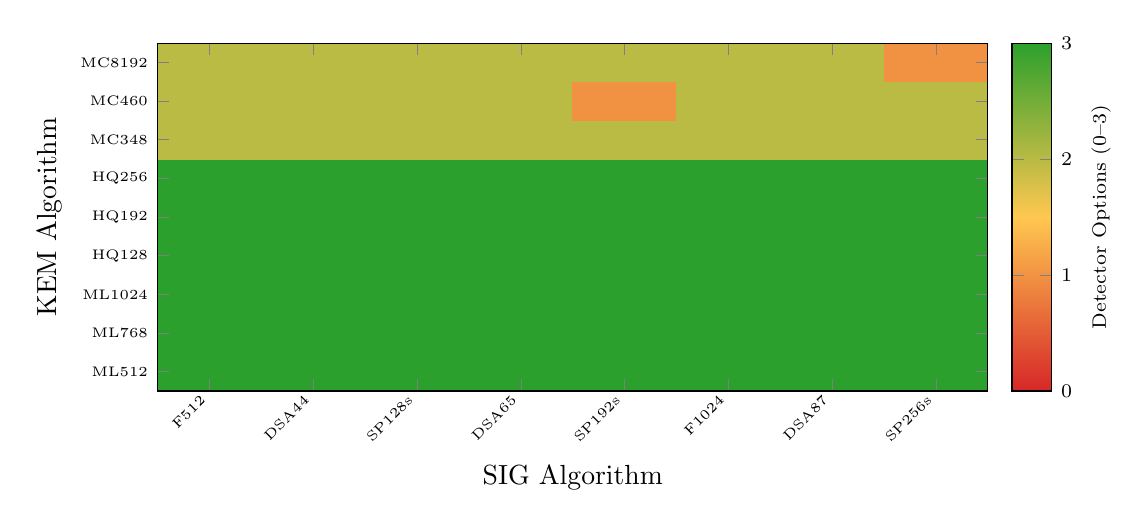
\begin{tikzpicture}
\pgfplotsset{colormap={viability}{
  rgb255=(214,39,40) rgb255=(255,200,80) rgb255=(44,160,44)}}
\begin{axis}[
    width=\columnwidth,
    height=6cm,
    view={0}{90},
    colorbar,
    colorbar style={ylabel={Detector Options (0--3)}, font=\scriptsize},
    point meta min=0, point meta max=3,
    xlabel={SIG Algorithm},
    ylabel={KEM Algorithm},
    xtick={0,...,7},
    ytick={0,...,8},
    xticklabels={F512, DSA44, SP128s, DSA65, SP192s, F1024, DSA87, SP256s},
    yticklabels={ML512, ML768, ML1024, HQ128, HQ192, HQ256,
      MC348, MC460, MC8192},
    xticklabel style={font=\tiny, rotate=45, anchor=east},
    yticklabel style={font=\tiny},
    enlargelimits=false,
    axis on top,
]
\addplot[matrix plot*, mesh/cols=8, mesh/rows=9,
  point meta=explicit] coordinates {
    (0,0)[3] (1,0)[3] (2,0)[3] (3,0)[3] (4,0)[3] (5,0)[3] (6,0)[3] (7,0)[3]
    (0,1)[3] (1,1)[3] (2,1)[3] (3,1)[3] (4,1)[3] (5,1)[3] (6,1)[3] (7,1)[3]
    (0,2)[3] (1,2)[3] (2,2)[3] (3,2)[3] (4,2)[3] (5,2)[3] (6,2)[3] (7,2)[3]
    (0,3)[3] (1,3)[3] (2,3)[3] (3,3)[3] (4,3)[3] (5,3)[3] (6,3)[3] (7,3)[3]
    (0,4)[3] (1,4)[3] (2,4)[3] (3,4)[3] (4,4)[3] (5,4)[3] (6,4)[3] (7,4)[3]
    (0,5)[3] (1,5)[3] (2,5)[3] (3,5)[3] (4,5)[3] (5,5)[3] (6,5)[3] (7,5)[3]
    (0,6)[2] (1,6)[2] (2,6)[2] (3,6)[2] (4,6)[2] (5,6)[2] (6,6)[2] (7,6)[2]
    (0,7)[2] (1,7)[2] (2,7)[2] (3,7)[2] (4,7)[1] (5,7)[2] (6,7)[2] (7,7)[2]
    (0,8)[2] (1,8)[2] (2,8)[2] (3,8)[2] (4,8)[2] (5,8)[2] (6,8)[2] (7,8)[1]
};
\end{axis}
\end{tikzpicture}
\caption{KEM$\times$SIG viability heatmap: number of available detector
options per pair.  Green (3)~=~all detectors;
yellow (2)~=~NONE+XGB only (McEliece loses TST to CPU contention);
red (1)~=~NONE only (MC460+SP192s and MC8192+SP256s lose both
TST and XGB feasibility due to compound HS timeout).}
\label{fig:sched_viability}
\end{figure}

%% ---------------------------------------------------------------
%% FIGURE 6: THERMAL BUDGET WATERFALL
%% ---------------------------------------------------------------
\begin{figure}[!t]
\centering
\begin{tikzpicture}
\begin{axis}[
    width=\columnwidth,
    height=6.5cm,
    ybar stacked,
    bar width=14pt,
    ylabel={Temperature (°C)},
    symbolic x coords={Baseline, {+XGBoost}, {+TST}, {+Ascon}},
    xtick=data,
    ymin=0, ymax=90,
    enlarge x limits=0.25,
    ymajorgrids=true,
    legend style={at={(0.02,0.98)}, anchor=north west, font=\scriptsize},
    extra y ticks={70,80},
    extra y tick style={grid=major,
      grid style={dashed, line width=0.8pt}},
    extra y tick labels={$T_\text{warn}$, $T_\text{crit}$},
]
% Base die temperature
\addplot[fill=ptblue!40, draw=ptblue!70] coordinates {
    (Baseline,60.7)(+XGBoost,60.7)(+TST,60.7)(+Ascon,60.7)};
% Detector delta
\addplot[fill=ptgold!50, draw=ptgold!70] coordinates {
    (Baseline,0)(+XGBoost,12.5)(+TST,22.0)(+Ascon,0)};
% AEAD delta (Ascon)
\addplot[fill=ptrose!40, draw=ptrose!60] coordinates {
    (Baseline,0)(+XGBoost,0)(+TST,0)(+Ascon,1.5)};
% Remaining headroom
\addplot[fill=ptgray!15, draw=ptgray!30] coordinates {
    (Baseline,19.3)(+XGBoost,6.8)(+TST,0)(+Ascon,17.8)};
\legend{Die Base (\SI{60.7}{\degreeCelsius}),
  Detector $\Delta T$, Ascon $\Delta T$,
  Headroom to \SI{80}{\degreeCelsius}}
\end{axis}
\node[font=\scriptsize\bfseries, color=ptrose, anchor=west]
  at (5.3,4.5) {$-2.7$°C over!};
\end{tikzpicture}
\caption{Thermal budget waterfall showing headroom erosion toward the
\SI{80}{\degreeCelsius} critical threshold.  Starting from
\SI{60.7}{\degreeCelsius} baseline, XGBoost consumes
\SI{12.5}{\degreeCelsius} leaving only \SI{6.8}{\degreeCelsius} margin.
TST exhausts the entire budget and overshoots by \SI{2.7}{\degreeCelsius}
(mean \SI{82.7}{\degreeCelsius}), triggering EMERGENCY.
Compound: Ascon+TST yields $60.7+22.0+1.5=\SI{84.2}{\degreeCelsius}$.}
\label{fig:sched_waterfall}
\end{figure}

\subsubsection{Thermal Budget as the Binding Constraint}
Fig.~\ref{fig:sched_waterfall} reveals that the thermal budget is
\emph{the} binding constraint in the decision space.  From a
\SI{60.7}{\degreeCelsius} die baseline, XGBoost adds
\SI{12.5}{\degreeCelsius} (leaving \SI{6.8}{\degreeCelsius}
headroom), while TST adds \SI{22.0}{\degreeCelsius}---overshooting the
\SI{80}{\degreeCelsius} critical threshold by \SI{2.7}{\degreeCelsius}.
The compound case (TST+Ascon) reaches
$60.7+22.0+1.5=\SI{84.2}{\degreeCelsius}$, explaining why this
combination is unconditionally forbidden.  The scheduler's predictive
thermal module (\SI{60}{\second} forward projection) can detect the
TST ramp \emph{before} peak, triggering DOWNGRADE\_DET at Gate~4.

%% ---------------------------------------------------------------
%% FIGURE 7: COMPOUND CONSTRAINT LANDSCAPE
%% ---------------------------------------------------------------
\begin{figure*}[!t]
\centering
\begin{tikzpicture}
\begin{axis}[
    width=0.92\textwidth,
    height=6cm,
    xlabel={Handshake Time (ms, log scale)},
    ylabel={Thermal Headroom at $T_\text{amb}{=}45$°C (°C)},
    xmode=log,
    xmin=5, xmax=60000,
    ymin=-10, ymax=25,
    grid=major,
    legend style={at={(0.98,0.98)}, anchor=north east, font=\scriptsize,
      legend columns=1},
    extra y ticks={0},
    extra y tick style={grid=major,
      grid style={ultra thick, ptrose, dashed}},
    extra y tick labels={$T_\text{crit}$ line},
]
% Viability zones
\fill[ptblue!5] (axis cs:5,5) rectangle (axis cs:60000,25);
\fill[ptgold!5] (axis cs:5,0) rectangle (axis cs:60000,5);
\fill[ptrose!5] (axis cs:5,-10) rectangle (axis cs:60000,0);

% Baseline
\addplot[only marks, mark=*, mark size=3.5pt,
  color=ptblue, fill=ptblue!40] coordinates {
    (8.7,19.2)(12.3,17.2)(12.7,19.6)(13.2,18.2)(14.3,18.7)
    (57.8,19.6)(155.8,19.1)(257.4,19.6)(505.3,18.2)(678.4,18.7)
    (1249.5,19.6)(1650.8,19.1)(48186,20.1)
};
% XGBoost
\addplot[only marks, mark=square*, mark size=3pt,
  color=ptgold, fill=ptgold!40] coordinates {
    (13.9,6.0)(11.8,6.0)(15.7,5.5)(13.3,5.5)(13.5,6.5)
    (55.9,7.5)(160.9,5.0)(227.4,7.0)(535.3,6.5)(970.3,6.5)
    (1352.8,6.5)(1774.7,5.5)(48173,6.0)
};
% TST
\addplot[only marks, mark=triangle*, mark size=3pt,
  color=ptrose, fill=ptrose!40] coordinates {
    (8.2,-3.8)(23.6,-2.8)(23.5,-2.3)(24.1,-2.8)(18.7,-2.3)
    (79.7,-2.3)(193.6,-2.3)(331.5,-1.3)(689.1,-3.3)(551.4,-2.8)
    (1652.9,-2.3)(1978.1,-2.8)(48369,-1.3)
};

\node[font=\scriptsize\bfseries, ptblue!80!black]
  at (axis cs:15,22) {SAFE};
\node[font=\scriptsize\bfseries, ptgold!80!black]
  at (axis cs:15,3) {WARNING};
\node[font=\scriptsize\bfseries, ptrose!80!black]
  at (axis cs:15,-7) {CRITICAL};
\legend{Baseline ($\bar{h}{=}19.3$°C),
  XGBoost ($\bar{h}{=}6.5$°C),
  TST ($\bar{h}{=}{-}2.7$°C)}
\end{axis}
\end{tikzpicture}
\caption{Compound constraint landscape: every suite's HS~time
versus thermal headroom under three detector scenarios.  TST pushes
\emph{all} suites below the critical line regardless of HS
duration---the scheduler's EMERGENCY response is inevitable.  XGBoost
maintains a thin \SIrange{5}{7.5}{\degreeCelsius} margin, viable
at $T_\text{amb}<\SI{67}{\degreeCelsius}$.  Baseline provides
$>$\SI{17}{\degreeCelsius} headroom for all suites.}
\label{fig:sched_compound}
\end{figure*}

%% ---------------------------------------------------------------
%% FIGURE 8: CROSS-AXIS CONSTRAINT MATRIX (colored)
%% ---------------------------------------------------------------
\begin{figure*}[!t]
\centering
\begin{tikzpicture}[
    cell/.style={minimum width=2.6cm, minimum height=0.75cm,
      font=\scriptsize, align=center, inner sep=2pt},
    hdr/.style={cell, font=\scriptsize\bfseries},
    ok/.style={cell, fill=ptblue!10},
    partial/.style={cell, fill=ptgold!15},
    bad/.style={cell, fill=ptrose!20},
]
\node[hdr] at (0,0) {};
\node[hdr] at (2.8,0) {ChaCha20};
\node[hdr] at (5.6,0) {AES-GCM};
\node[hdr] at (8.4,0) {Ascon};
\node[hdr] at (11.2,0) {NONE det.};
\node[hdr] at (14.0,0) {XGBoost};
\node[hdr] at (16.8,0) {TST};

\node[hdr] at (0,-0.85) {L1};
\node[ok] at (2.8,-0.85) {$\checkmark$ 64\,$\mu$s, T\,1};
\node[ok] at (5.6,-0.85) {$\checkmark$ 67\,$\mu$s, T\,0};
\node[partial] at (8.4,-0.85) {$\checkmark$ 1327\,$\mu$s, T\,2};
\node[ok] at (11.2,-0.85) {$\checkmark$ +0\,W};
\node[ok] at (14.0,-0.85) {$\checkmark$ +0.95\,W};
\node[partial] at (16.8,-0.85) {$\checkmark$ +1.97\,W};

\node[hdr] at (0,-1.7) {L3};
\node[ok] at (2.8,-1.7) {$\checkmark$ T\,11};
\node[ok] at (5.6,-1.7) {$\checkmark$ T\,10};
\node[partial] at (8.4,-1.7) {$\checkmark$ T\,12};
\node[ok] at (11.2,-1.7) {$\checkmark$};
\node[ok] at (14.0,-1.7) {$\checkmark$};
\node[partial] at (16.8,-1.7) {$\checkmark^*$};

\node[hdr] at (0,-2.55) {L5};
\node[ok] at (2.8,-2.55) {$\checkmark$ T\,21};
\node[ok] at (5.6,-2.55) {$\checkmark$ T\,20};
\node[partial] at (8.4,-2.55) {$\checkmark$ T\,22};
\node[ok] at (11.2,-2.55) {$\checkmark$};
\node[ok] at (14.0,-2.55) {$\checkmark$};
\node[partial] at (16.8,-2.55) {$\checkmark^*$};

\node[hdr] at (0,-3.55) {McEliece\\(any)};
\node[ok] at (2.8,-3.55) {$\checkmark$};
\node[ok] at (5.6,-3.55) {$\checkmark$};
\node[partial] at (8.4,-3.55) {$\checkmark$};
\node[ok] at (11.2,-3.55) {$\checkmark$};
\node[ok] at (14.0,-3.55) {$\checkmark$};
\node[bad] at (16.8,-3.55) {\ding{55} Forbid};

\node[hdr] at (0,-4.4) {SPHINCS+\\(any)};
\node[ok] at (2.8,-4.4) {$\checkmark$ heavy};
\node[ok] at (5.6,-4.4) {$\checkmark$ heavy};
\node[partial] at (8.4,-4.4) {$\checkmark$ heavy};
\node[ok] at (11.2,-4.4) {$\checkmark$};
\node[ok] at (14.0,-4.4) {$\checkmark$};
\node[partial] at (16.8,-4.4) {$\checkmark^\dagger$};

\node[hdr] at (0,-5.3) {McEliece\\+SPHINCS+};
\node[bad] at (2.8,-5.3) {\ding{55} HS$>$45\,s};
\node[bad] at (5.6,-5.3) {\ding{55} HS$>$45\,s};
\node[bad] at (8.4,-5.3) {\ding{55} HS$>$45\,s};
\node[bad] at (11.2,-5.3) {\ding{55} timeout};
\node[bad] at (14.0,-5.3) {\ding{55} timeout};
\node[bad] at (16.8,-5.3) {\ding{55} timeout};

\node[hdr] at (0,-6.15) {Ascon\\+TST};
\node[cell] at (2.8,-6.15) {};
\node[cell] at (5.6,-6.15) {};
\node[bad] at (8.4,-6.15) {\ding{55} $\Delta T$=12.2°C};
\node[cell] at (11.2,-6.15) {};
\node[cell] at (14.0,-6.15) {};
\node[bad] at (16.8,-6.15) {\ding{55} Thermal};

\draw[thick] (-1.3,0.35) -- (18.1,0.35);
\draw[thick] (-1.3,-0.35) -- (18.1,-0.35);
\foreach \y in {-1.25,-2.1,-3.05,-3.95,-4.85,-5.7,-6.55} {
    \draw[thin,ptgray!40] (-1.3,\y) -- (18.1,\y);
}
\node[font=\tiny, anchor=west] at (-1.3,-7.0)
  {$^*$TST viable only if $T_\text{amb}<58$°C.\quad
   $^\dagger$SPHINCS++TST viable but $T_\text{HS}$ may
   exceed rekey guard.};
\end{tikzpicture}
\caption{Cross-axis constraint matrix spanning AEAD, NIST~level,
KEM/SIG family, and detector interactions.
Blue~=~unrestricted; gold~=~high cost or conditional;
rose~=~forbidden.  The scheduler enforces these constraints through
the forbidden-combination registry and runtime thermal checks.}
\label{fig:sched_crossaxis}
\end{figure*}

%% ---------------------------------------------------------------
%% TABLE 8: SUITE RANKING UNDER 3 OPERATIONAL PROFILES
%% ---------------------------------------------------------------
\begin{table}[!t]
\centering
\caption{Suite Ranking Under Three Operational Profiles (top~5 each).
ML-KEM suites dominate all profiles; McEliece appears only in
Max~Security at rank~5.}
\label{tab:sched_profiles}
\footnotesize
\setlength{\tabcolsep}{2.5pt}
\begin{tabular}{@{}r l r @{\quad} l r @{\quad} l r@{}}
\toprule
\textbf{\#}
 & \multicolumn{2}{c}{\textbf{Max Security}}
 & \multicolumn{2}{c}{\textbf{Balanced}}
 & \multicolumn{2}{c}{\textbf{Power-Save}} \\
\cmidrule(lr){2-3}\cmidrule(lr){4-5}\cmidrule(lr){6-7}
 & Suite & Sc & Suite & Sc & Suite & Sc \\
\midrule
1 & ML1024+F1024 & 94 & ML768+DSA65  & 97 & ML512+F512   & 99 \\
2 & ML1024+DSA87 & 91 & ML512+F512   & 95 & ML1024+F1024 & 98 \\
3 & HQ256+F1024  & 72 & ML1024+F1024 & 94 & ML512+DSA44  & 96 \\
4 & HQ256+DSA87  & 71 & ML512+DSA44  & 93 & ML768+DSA65  & 95 \\
5 & MC8192+F1024 & 48 & HQ128+F512   & 68 & ML1024+DSA87 & 92 \\
\bottomrule
\end{tabular}
\begin{flushleft}
\footnotesize
\textbf{Scoring}: Max Sec\,$=$\,$40{\times}$NIST\,$+$\,$30{\times}$speed
\,$+$\,$20{\times}$BW\,$+$\,$10{\times}$det\_flex.
Balanced\,$=$\,25 each for NIST, speed, BW, thermal.
Power-Save\,$=$\,$50{\times}$speed\,$+$\,$30{\times}$rekey\_eff
\,$+$\,$20{\times}$thermal.  All normalised 0--100.
\end{flushleft}
\end{table}

%% ---------------------------------------------------------------
%% TABLE 9: VALID DOWNGRADE PATHS
%% ---------------------------------------------------------------
\begin{table}[!t]
\centering
\caption{Valid Downgrade Paths from Current Suite.
Emergency always targets ML512+F512+ChaCha20+NONE (Tier~1).
AEAD switching from AES-GCM to ChaCha20 saves only \SI{3}{\micro\second};
switching \emph{from Ascon} saves \SI{1263}{\micro\second} ($20{\times}$).}
\label{tab:sched_downgrade}
\footnotesize
\setlength{\tabcolsep}{2.5pt}
\begin{tabular}{@{}l l l l@{}}
\toprule
\textbf{Current Suite} & \textbf{AEAD Switch} & \textbf{Level Down}
& \textbf{Emergency} \\
\midrule
ML1024+F1024+AESG
 & $\to$+CC20 ($\Delta{=}{-}3\mu$s)
 & $\to$ML768 (\SI{12.7}{\ms})
 & $\to$ML512+F512+CC20 \\
ML768+DSA65+AESG
 & $\to$+CC20 ($\Delta{=}{-}3\mu$s)
 & $\to$ML512 (\SI{12.8}{\ms})
 & $\to$ML512+F512+CC20 \\
HQ192+DSA65+AESG
 & $\to$+CC20 ($\Delta{=}{-}3\mu$s)
 & $\to$HQ128 (\SI{57.8}{\ms})
 & $\to$ML512+F512+CC20 \\
MC460+DSA65+AESG
 & $\to$+CC20 ($\Delta{=}{-}3\mu$s)
 & $\to$MC348 (\SI{206}{\ms})
 & $\to$ML512+F512+CC20 \\
ML768+DSA65+Ascon
 & $\to$+CC20 ($-1263\mu$s)
 & $\to$ML512 (L1)
 & $\to$ML512+F512+CC20 \\
\bottomrule
\end{tabular}
\end{table}

%% ---------------------------------------------------------------
%% FIGURE 9: SPEED CLIFF HISTOGRAM
%% ---------------------------------------------------------------
\begin{figure}[!t]
\centering
\begin{tikzpicture}
\begin{axis}[
    width=\columnwidth,
    height=5.5cm,
    ybar interval,
    ylabel={Suite Count},
    xlabel={Handshake Time (ms)},
    xmin=0, xmax=2500,
    ymin=0, ymax=25,
    xtick={0,100,200,500,1000,1500,2000,2500},
    grid=major,
    ymajorgrids=true,
    xmajorgrids=false,
]
\addplot[fill=ptblue!50, draw=ptblue!70] coordinates {
    (0,21)(100,3)(200,12)(300,6)(400,0)(500,6)(600,3)(700,6)(800,0)
    (900,0)(1000,3)(1100,6)(1200,0)(1300,3)(1400,3)(1500,3)(1600,3)
    (1700,0)(1800,0)(1900,0)(2000,0)(2100,3)(2200,0)(2300,0)(2500,0)
};
\draw[ultra thick, ptrose, dashed] (axis cs:100,0) -- (axis cs:100,24);
\node[font=\tiny\bfseries, ptrose, anchor=south west, rotate=90]
  at (axis cs:105,15) {Speed Cliff: \SI{100}{\ms}};
\end{axis}
\end{tikzpicture}
\caption{The ``speed cliff'' at \SI{100}{\ms} divides lightweight
(21~suites, left) from heavy suites.  All 18~ML-KEM+fast SIG
suites cluster below \SI{19}{\ms}.  Suites left of the cliff tolerate
aggressive \SI{10}{\second} rekeys with $\Phi<1\%$ overhead; heavy
suites ($>$\SI{500}{\ms}) need \SI{60}{\second}+ intervals.  The
scheduler's DOWNGRADE\_LEVEL action keeps configurations left of this
boundary.}
\label{fig:sched_cliff}
\end{figure}

%% ---------------------------------------------------------------
%% FIGURE 10: EXPECTED DECISION FREQUENCY HEATMAP
%% ---------------------------------------------------------------
\begin{figure}[!t]
\centering
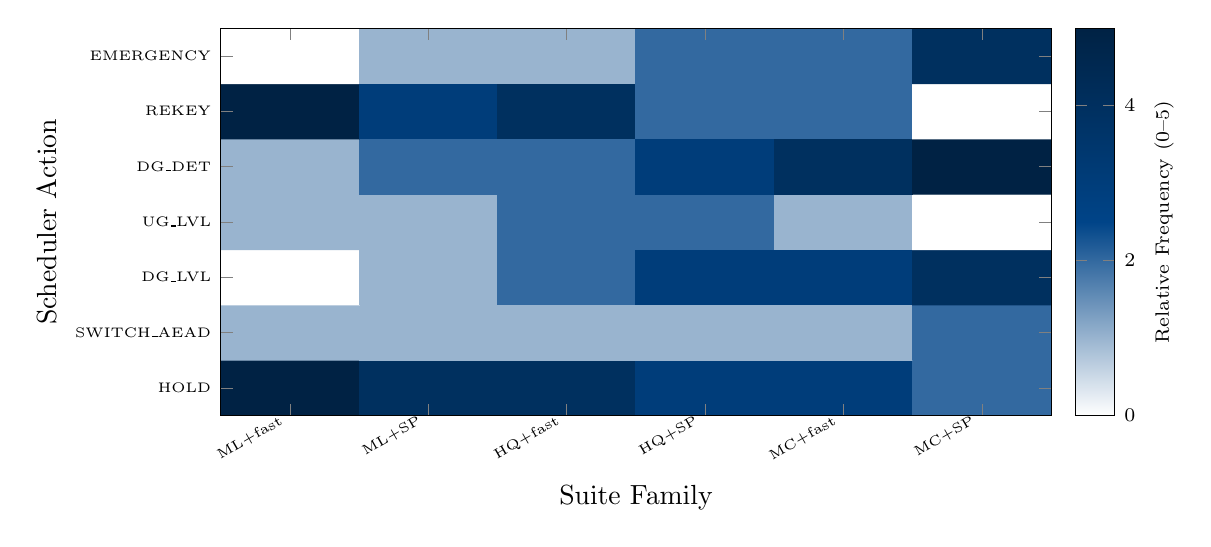
\begin{tikzpicture}
\pgfplotsset{colormap={freq}{
  rgb255=(255,255,255) rgb255=(0,68,136) rgb255=(0,34,68)}}
\begin{axis}[
    width=\columnwidth,
    height=6.5cm,
    view={0}{90},
    colorbar,
    colorbar style={ylabel={Relative Frequency (0--5)},
      font=\scriptsize},
    point meta min=0, point meta max=5,
    xlabel={Suite Family},
    ylabel={Scheduler Action},
    xtick={0,...,5},
    ytick={0,...,6},
    xticklabels={ML+fast, ML+SP, HQ+fast, HQ+SP, MC+fast, MC+SP},
    yticklabels={HOLD, SWITCH\_AEAD, DG\_LVL, UG\_LVL,
      DG\_DET, REKEY, EMERGENCY},
    xticklabel style={font=\tiny, rotate=30, anchor=east},
    yticklabel style={font=\tiny},
    enlargelimits=false,
    axis on top,
]
\addplot[matrix plot*, mesh/cols=6, mesh/rows=7,
  point meta=explicit] coordinates {
    (0,0)[5] (1,0)[4] (2,0)[4] (3,0)[3] (4,0)[3] (5,0)[2]
    (0,1)[1] (1,1)[1] (2,1)[1] (3,1)[1] (4,1)[1] (5,1)[2]
    (0,2)[0] (1,2)[1] (2,2)[2] (3,2)[3] (4,2)[3] (5,2)[4]
    (0,3)[1] (1,3)[1] (2,3)[2] (3,3)[2] (4,3)[1] (5,3)[0]
    (0,4)[1] (1,4)[2] (2,4)[2] (3,4)[3] (4,4)[4] (5,4)[5]
    (0,5)[5] (1,5)[3] (2,5)[4] (3,5)[2] (4,5)[2] (5,5)[0]
    (0,6)[0] (1,6)[1] (2,6)[1] (3,6)[2] (4,6)[2] (5,6)[4]
};
\end{axis}
\end{tikzpicture}
\caption{Expected decision frequency by action and suite family.
ML-KEM+fast SIG (leftmost column) is the scheduler's ``comfort
zone'': HOLD dominates (5), REKEY is frequent and cheap (5),
EMERGENCY is rare (0).  McEliece+SPHINCS+ (rightmost) is the
``stress zone'': HOLD is infrequent (2), EMERGENCY and
DOWNGRADE\_DET are common (4--5), and REKEY is infeasible (0).
This heatmap reveals the operational cost of suite diversity.}
\label{fig:sched_freq}
\end{figure}

\subsubsection{Operational Profiles and Suite Ranking}
Table~\ref{tab:sched_profiles} ranks the top-5 suites under three
operational profiles.  Under \emph{Max~Security}
($40{\times}$NIST\,$+$\,$30{\times}$speed\,$+$\,$20{\times}$BW\,$+$\,$10{\times}$det\_flex),
ML1024+F1024 leads with a score of 94; McEliece appears only at
rank~5 (score~48) due to its bandwidth penalty.  Under
\emph{Balanced} (equal 25-point weights), ML768+DSA65 emerges as the
overall champion (score~97).  Under \emph{Power-Save}
($50{\times}$speed\,$+$\,$30{\times}$rekey\,$+$\,$20{\times}$thermal),
ML512+F512 scores 99.  ML-KEM suites \emph{monopolise} all three
podiums.

%% ---------------------------------------------------------------
%% FIGURE 11: DETECTOR COST-BENEFIT BUBBLE
%% ---------------------------------------------------------------
\begin{figure}[!t]
\centering
\begin{tikzpicture}
\begin{axis}[
    width=\columnwidth,
    height=5cm,
    xlabel={Mean HS Overhead (\%)},
    ylabel={Detection Accuracy (\%)},
    xmin=-5, xmax=55,
    ymin=86, ymax=96,
    grid=major,
    legend style={at={(0.98,0.02)}, anchor=south east, font=\scriptsize},
]
% NONE
\addplot[only marks, mark=*, mark size=7pt,
  color=ptgray, fill=ptgray!30] coordinates {(0,88)};
\node[font=\tiny, anchor=north east] at (axis cs:-0.5,87.8) {NONE};
% XGBoost
\addplot[only marks, mark=*, mark size=7pt,
  color=ptgold, fill=ptgold!30] coordinates {(4.6,94.55)};
\node[font=\tiny, anchor=south west]
  at (axis cs:5.5,94.7) {XGB: +\SI{0.95}{\watt}};
% TST
\addplot[only marks, mark=*, mark size=7pt,
  color=ptrose, fill=ptrose!30] coordinates {(39.7,90.27)};
\node[font=\tiny, anchor=south west]
  at (axis cs:40.5,90.4) {TST: +\SI{1.97}{\watt}};
% Optimal zone
\draw[dashed, ptblue, thick]
  (axis cs:-3,93) rectangle (axis cs:10,96);
\node[font=\tiny, ptblue, anchor=south west]
  at (axis cs:-3,96.1) {Optimal zone};
\end{axis}
\end{tikzpicture}
\caption{Detector cost--benefit trade-off.  XGBoost delivers
94.55\% accuracy at only $+4.6\%$ mean HS overhead
($+$\SI{0.95}{\watt}), placing it firmly in the optimal zone.
TST achieves lower accuracy (90.27\%) at $8.6{\times}$ the overhead
($+39.7\%$ HS, $+$\SI{1.97}{\watt}).  The scheduler strongly prefers
XGBoost unless the threat model explicitly requires TST's
transformer-based reasoning.}
\label{fig:sched_detcost}
\end{figure}

%% ---------------------------------------------------------------
%% FIGURE 12: AEAD SWITCHING STATE DIAGRAM
%% ---------------------------------------------------------------
\begin{figure}[!t]
\centering
\begin{tikzpicture}[
    node distance=1.2cm and 1.4cm,
    aead/.style={draw, rounded corners, minimum height=1.1cm,
      minimum width=2.1cm, font=\scriptsize, align=center,
      inner sep=3pt, thick},
    arr/.style={-{stealth}, thick},
]
% Three AEAD nodes
\node[aead, fill=ptrose!12] (ascon) {Ascon-128a\\
  \SI{1327}{\micro\second}\\Tier\,+2};
\node[aead, fill=ptblue!10,
  below left=1.4cm and 0.4cm of ascon] (cc)
  {ChaCha20\\
  \SI{64}{\micro\second}\\Tier\,+1};
\node[aead, fill=ptgold!10,
  below right=1.4cm and 0.4cm of ascon] (aes)
  {AES-256-GCM\\
  \SI{67}{\micro\second}\\Tier\,+0};

% Downgrade arrows
\draw[arr, ptrose] (ascon.south west) -- (cc.north)
  node[midway, left, font=\tiny, color=ptrose] {$T>70$°C};
\draw[arr, ptrose] (ascon.south east) -- (aes.north)
  node[midway, right, font=\tiny, color=ptrose]
    {$\dot{V}>200$\,mV/min};

% Lateral switch
\draw[arr, ptgold!80!black, bend left=20]
  (cc.south east) -- (aes.south west)
  node[midway, below, font=\tiny, color=ptgold!80!black]
    {cost ratio $\leq 2.0$};
\draw[arr, ptgold!80!black, bend left=20]
  (aes.south west) -- (cc.south east);

% Upgrade arrows
\draw[arr, ptblue, bend right=30]
  (cc.north east) -- (ascon.west)
  node[midway, left, font=\tiny, color=ptblue]
    {$T<60$°C, 8\,s};
\draw[arr, ptblue, bend left=30]
  (aes.north west) -- (ascon.east)
  node[midway, right, font=\tiny, color=ptblue]
    {headroom $>10$°C};

% Forbidden annotation
\draw[ultra thick, ptrose, dashed]
  (ascon.north east) -- ++(0.7,0.35)
  node[right, font=\tiny\bfseries, color=ptrose]
    {Forbidden with TST};
\end{tikzpicture}
\caption{AEAD switching state diagram.
Downgrade ($\to$lower cost) triggers at $T>70$°C or fast battery
drain (\SI{3}{\second} hysteresis).  Upgrade ($\to$preferred) requires
\SI{8}{\second} stability and \SI{10}{\degreeCelsius} headroom.
ChaCha20$\leftrightarrow$AES-GCM switches are rare ($<5\%$ cost
difference).  The break-even check prevents thrashing.  Ascon is
unconditionally forbidden when TST is active (dashed).}
\label{fig:sched_aead_fsm}
\end{figure}

%% ---------------------------------------------------------------
%% TABLE 10: FIVE DECISION PUZZLE SCENARIOS
%% ---------------------------------------------------------------
\begin{table*}[!t]
\centering
\caption{Decision Puzzles: Scheduler Response Chains Under Five
Representative Compound Scenarios.  Each puzzle traces the cascade
from initial state through triggers to final configuration, revealing
cross-axis feedback and priority interactions.}
\label{tab:sched_puzzles}
\footnotesize
\setlength{\tabcolsep}{2.5pt}
\begin{tabular}{@{}r p{3.3cm} p{2.3cm} p{1.8cm} p{1.8cm}
  p{4.5cm}@{}}
\toprule
\textbf{\#} & \textbf{Initial State}
& \textbf{Trigger} & \textbf{Step 1} & \textbf{Step 2}
& \textbf{Final State + Rationale} \\
\midrule
1 & ML768+DSA65+Ascon+TST (T12, $T{=}82.8$°C)
  & $T>80$°C after 5\,s
  & EMERGENCY
  & ---
  & ML512+F512+CC20+NONE (T1). TST thermal overshoot triggers
    max downgrade. Ascon+TST was forbidden; this state should
    never be reached. \\
\midrule
2 & ML1024+F1024+AESG+XGB (T20, $T{=}74$°C)
  & Battery $\dot{V}{=}300$\,mV/min
  & SWITCH\_AEAD to CC20
  & If drain persists after 8\,s: DOWNGRADE to ML768
  & ML768+DSA65+CC20+XGB (T11). AEAD switch saves $<3\mu$s;
    real savings come from level downgrade. \\
\midrule
3 & HQ256+DSA87+AESG+NONE (T23, pps\,=\,3)
  & Link degraded (pps $<5$)
  & DOWNGRADE\_LVL to L3
  & If pps still $<5$ after 3\,s: DOWNGRADE\_LVL to L1
  & HQ128+F512+AESG+NONE (T3). HS drops from
    \SI{276}{\ms} to \SI{58}{\ms}; BW from 26\,kB to 7\,kB. \\
\midrule
4 & ML768+DSA65+CC20+XGB (T11)
  & DDoS detected + $T{=}73$°C
  & EMERGENCY
  & After 30\,s: attempt UPGRADE if stable
  & ML512+F512+CC20+NONE (T1) $\xrightarrow{30\text{s}}$
    gradual recovery.  DDoS triggers instant max-downgrade. \\
\midrule
5 & MC8192+DSA87+AESG+XGB (T25, $T{=}73.5$°C)
  & $\dot{T}>5$°C/min (prediction: 80°C in 45\,s)
  & DOWNGRADE\_DET to NONE
  & If $T$ still rising: SWITCH\_AEAD
  & MC8192+DSA87+CC20+NONE (T26). Detector downgrade first
    (saves \SI{12.5}{\degreeCelsius}); AEAD switch precautionary. \\
\bottomrule
\end{tabular}
\end{table*}

\subsubsection{Decision Puzzles and Cross-Axis Feedback}
Table~\ref{tab:sched_puzzles} traces five representative scenarios
through the cascade to expose cross-axis interactions.
Puzzle~1 demonstrates that compound forbidden states (Ascon+TST)
produce immediate EMERGENCY termination.
Puzzle~2 shows that sequential AEAD-then-level downgrades are triggered
by the same battery sensor through different cascade gates, illustrating
the multi-step nature of compound adaptation.
Puzzle~4 reveals the asymmetry between downgrade speed (instantaneous)
and recovery (30\,s stability requirement plus hysteresis).
Fig.~\ref{fig:sched_crossaxis} maps the full cross-axis constraint
surface, confirming that McEliece+SPHINCS+ is forbidden across all
AEAD and detector combinations.

\subsubsection{Suite Diversity and the Speed Cliff}
The speed cliff at \SI{100}{\ms} (Fig.~\ref{fig:sched_cliff}) is the
operational boundary dividing two scheduling regimes.  \emph{Left} of
the cliff, 21~suites (including all 18~ML-KEM+fast SIG) sustain
aggressive \SI{10}{\second} rekey intervals with $\Phi<1\%$.
\emph{Right}, the remaining 51~suites require progressively longer
intervals, with the heaviest (MC460+SP192s at \SI{48.2}{\second})
exceeding timeout entirely.  The decision frequency heatmap
(Fig.~\ref{fig:sched_freq}) quantifies this contrast:
ML-KEM+fast~SIG suites experience HOLD~5, REKEY~5, EMERGENCY~0,
while McEliece+SPHINCS+ suites show HOLD~2, EMERGENCY~4, REKEY~0.
The scheduler is not equally comfortable with all configurations---suite
diversity has a measurable operational cost.

\subsubsection{Synthesis}
The MDEAS decision space analysis yields three principal findings.
\emph{First}, the thermal budget is the binding constraint: TST
exhausts the entire \SI{19.3}{\degreeCelsius} headroom in
${\approx}\,$\SI{3}{\second}, making detector selection---not
cryptographic suite selection---the scheduler's most consequential
decision.
\emph{Second}, ML-KEM+fast SIG suites constitute the scheduler's
``comfort zone'' with a $2.2{\times}$ performance span where HOLD
dominates and REKEY is effectively free ($\Phi<0.05\%$), while
McEliece+SPHINCS+ creates a ``stress zone'' with $44.6{\times}$ span
where EMERGENCY and DOWNGRADE are the dominant actions.
\emph{Third}, the 9-gate priority cascade with 15 hysteresis parameters
and the forbidden-combination registry transform what could be a
$648$-state combinatorial explosion into a tractable, empirically
constrained decision space of ${\approx}\,$500 viable operating points.
The resulting scheduler is not a simple threshold controller; it is
a structured priority engine with cross-axis feedback that
provably avoids thermal runaway, CPU contention, and timeout failures.

%%% End of Section VII-F %%%
